\chapter{Requirements}

\section{Use cases}

As with all requirements specifications, a good place to begin was to create various use case diagrams representing the roles in the system and the actions they ought to be able to perform. By doing so, it would also be possible to derive common classes and actions by examining similar or duplicating use case scenarios.

\subsection{Registration}

\begin{figure}[h!]
  \centering
    \ifimages
    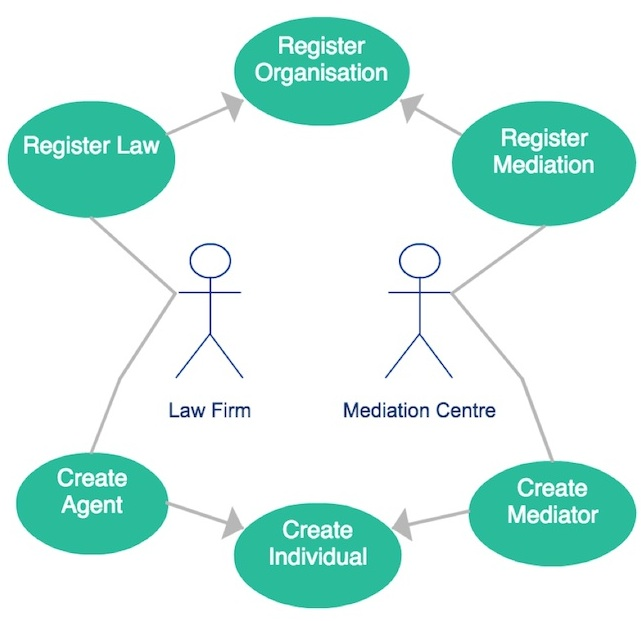
\includegraphics[width=\textwidth]{use_case--registration}
    \fi
  \caption{Use case diagram showing registration feature}
  \label{uml:useCase:registration}
\end{figure}

Authorised individuals should be allowed to register accounts representing their company (be it a law firm or mediation centre), and that within that organised account they should be able to register individual accounts, which should be agents or mediators depending on the organisation type.

Figure~\ref{uml:useCase:registration} shows this in terms of the law firms and mediation centres. In both the organisational and individual registration, a generalised action has been added which these more specific actions can extend or implement, showing where it might be possible to use a common class or database table to accomplish both goals.

\subsection{Disputes}

\begin{figure}[h!]
  \centering
    \ifimages
    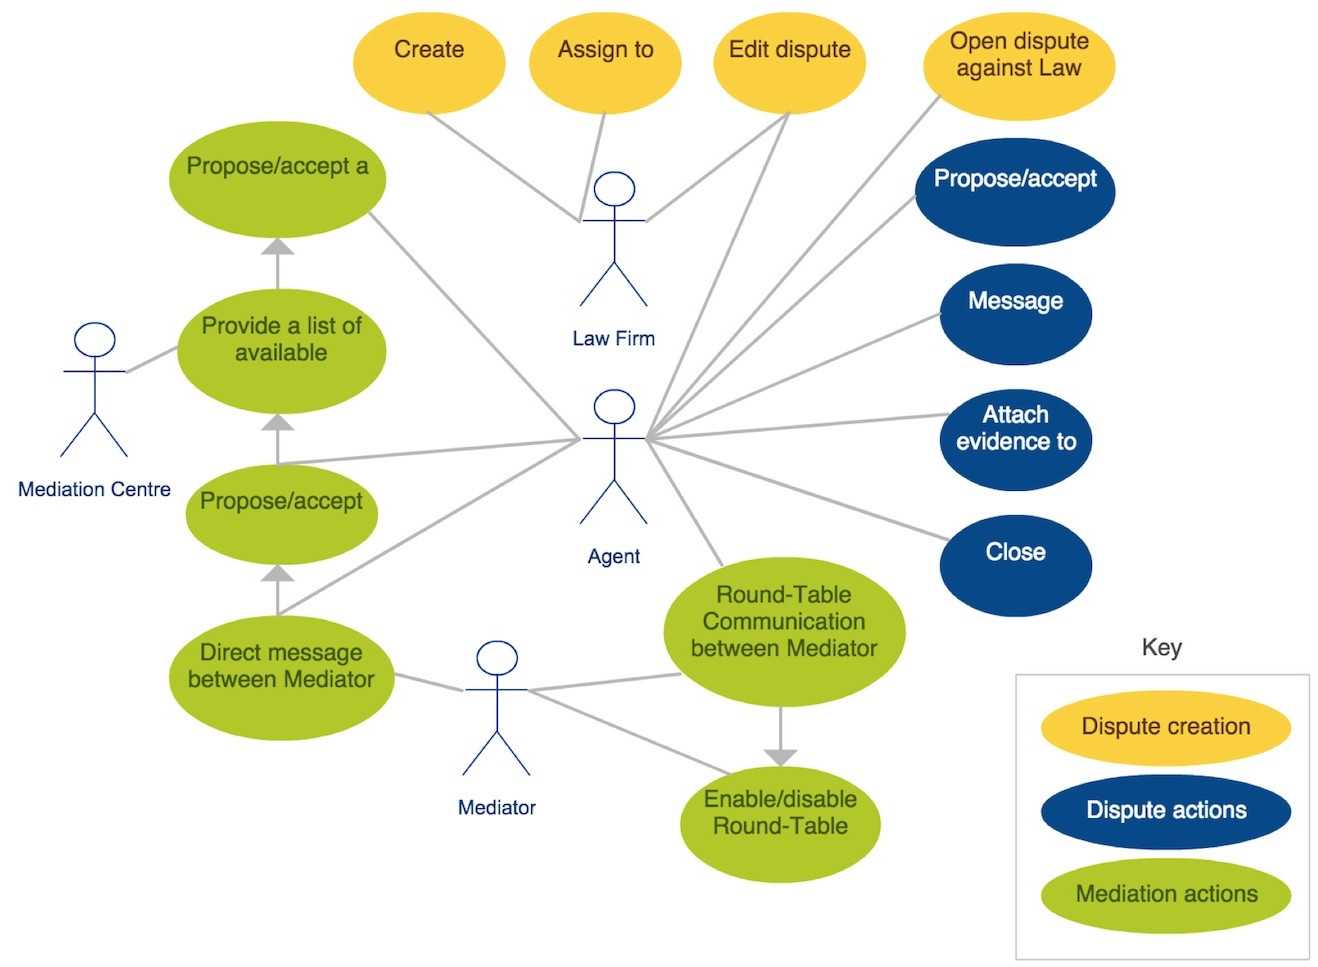
\includegraphics[width=\textwidth]{use_case--disputes}
    \fi
  \caption{Use case diagram showing actions available in a dispute}
  \label{uml:useCase:disputes}
\end{figure}

Figure~\ref{uml:useCase:disputes} shows the roles and actions involved in the creation, mediation and closing of a dispute.

Only law firms can create new disputes. There is then some back-and-forth assignment between law firms and agents until both sides of a dispute are represented by different agents. This is identified as being the ``dispute creation" stage.

Inside a dispute, agents should be able to negotiate the dispute lifespan, exchange messages and evidence, and should have the freedom to close a dispute. In a best-case scenario, this is all that is required to successfully resolve a dispute. This is known as the ``dispute" stage.

Should it be required, an agent can propose mediation, and there is a defined process of administration between the agents and mediation centre required to get the dispute `in mediation'. Once in this state, the agents can communicate only through the mediator, unless the mediator feels the dispute is close to resolution and decides to enable round-table communication.

\subsection{Miscellaneous}

\begin{figure}[h!]
  \centering
    \ifimages
    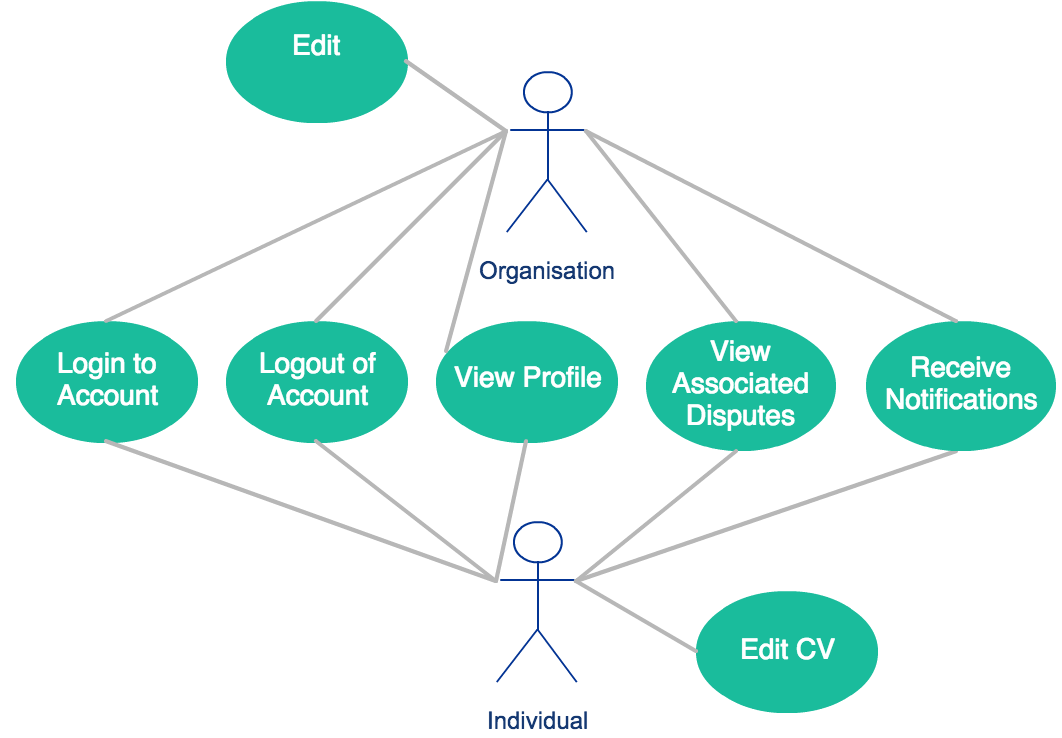
\includegraphics[width=\textwidth]{use_case--miscellaneous}
    \fi
  \caption{Use case diagram demonstrating other miscellaneous requirements}
  \label{uml:useCase:miscellaneous}
\end{figure}

Other, lesser elements of functionality are shown by the miscellaneous UML diagram in figure~\ref{uml:useCase:miscellaneous}. For example, agents should be able to peruse a mediator's CV before making a decision as to which mediator to opt for. This suggests a ``view profile" facility, with custom fields for the CV, which could be as simple as a HTML textarea or as complicated as an integrated PDF uploader and viewer.

Given the tight deadline of the project and the scale of the system, coupled with the high priority of demonstrating some maritime collision logic, it was decided that these miscellaneous features should be kept as simple as possible.

\section{Dispute process}

Although the use case diagrams describe the features required by the system, they do not clarify when those features should or should not be available. An early meeting with the client, Dr Constantina Sampani, made it clear that there was a very specific workflow that a dispute should follow.

\begin{figure}[h!]
  \centering
    \ifimages
    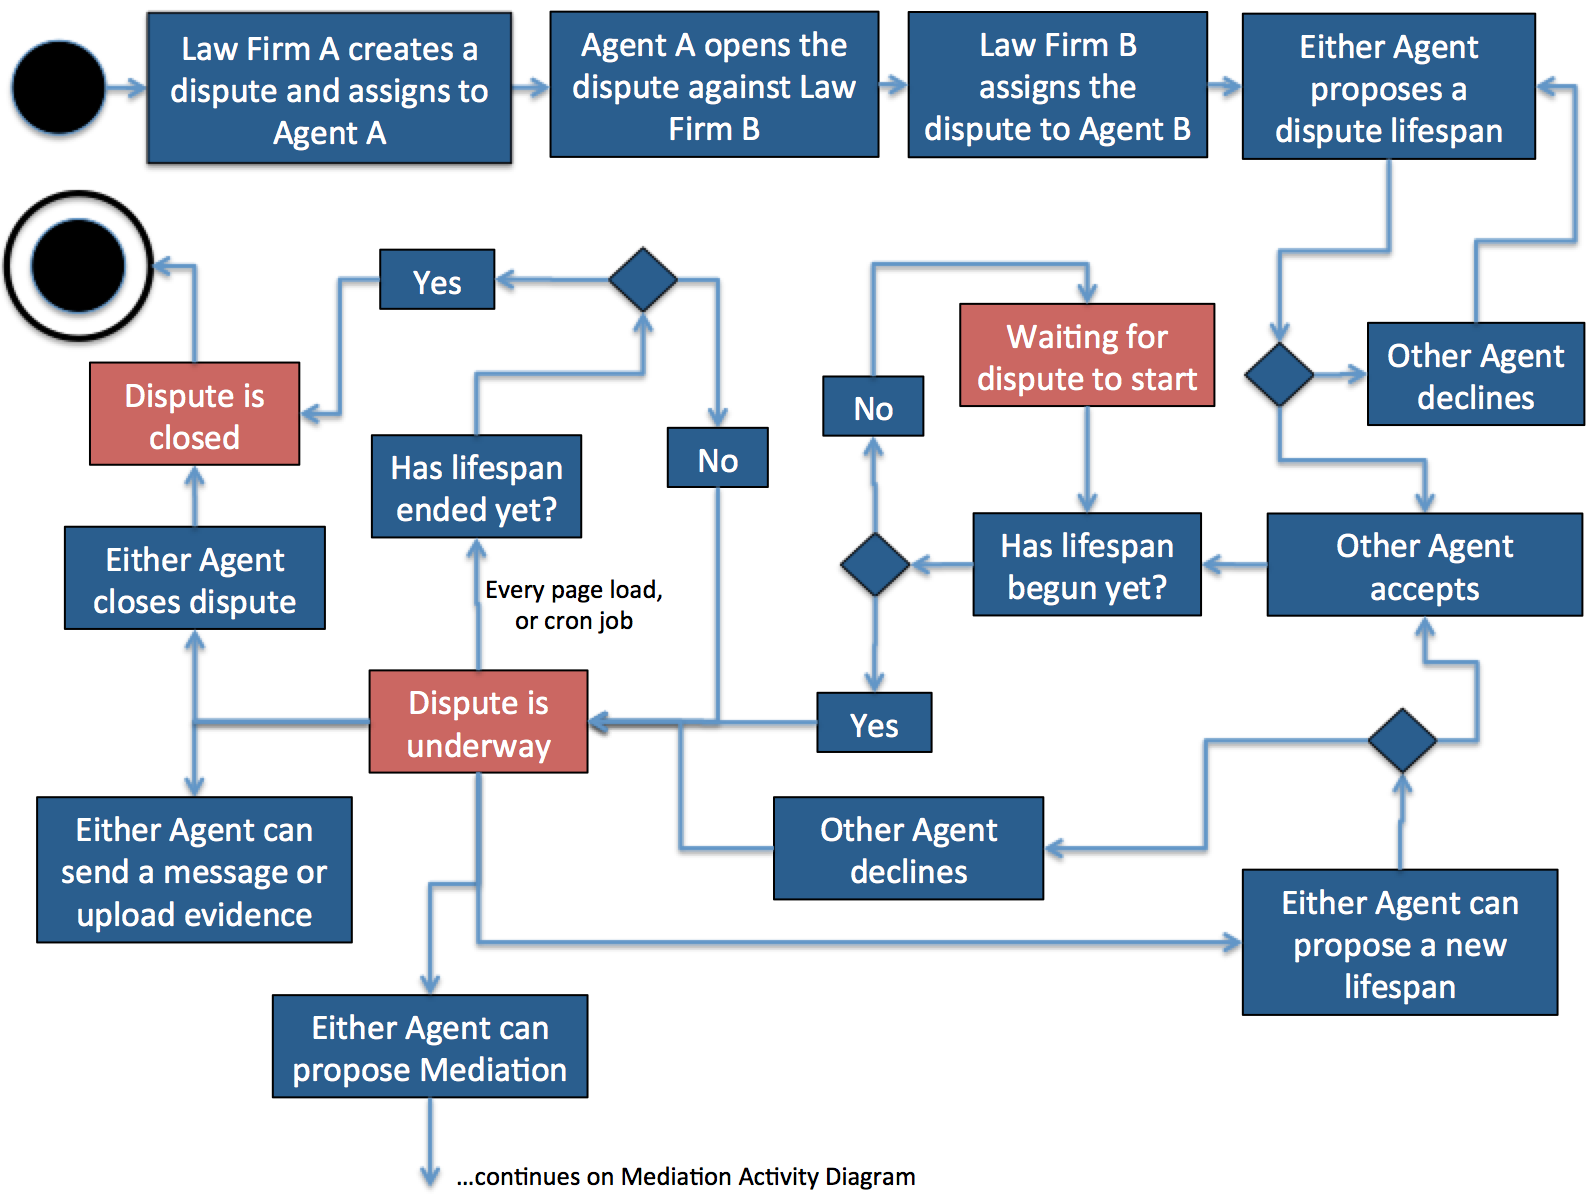
\includegraphics[width=\textwidth]{dispute_process}
    \fi
  \caption{Activity diagram showing the workflow required in creating a dispute}
  \label{uml:activity:dispute}
\end{figure}

Figure~\ref{uml:activity:dispute} shows the creation of a dispute and the features that become available to the agents when the dispute has been initialised.

The red boxes indicate the current state of the dispute. These helped later on when designing the classes involved in the state pattern.

\begin{figure}[h!]
  \centering
    \ifimages
    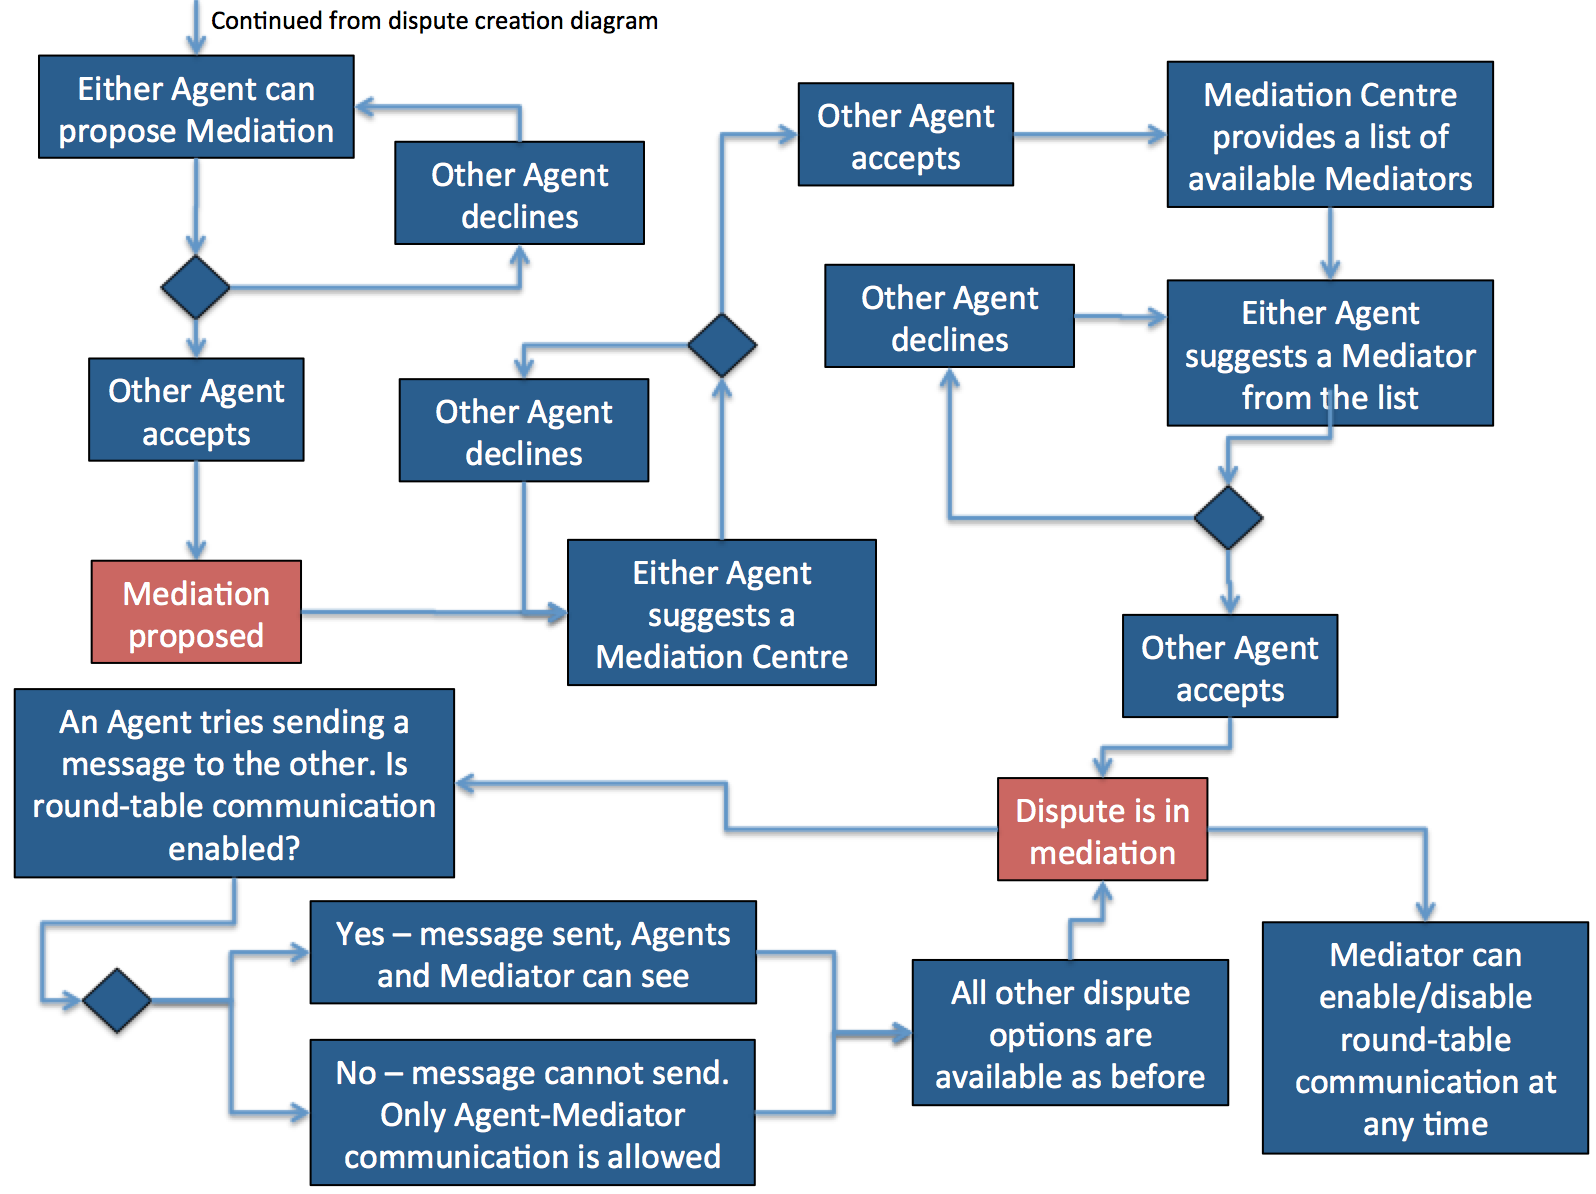
\includegraphics[width=\textwidth]{dispute_process--mediation}
    \fi
  \caption{Activity diagram showing the workflow involved in getting a dispute into mediation}
  \label{uml:activity:mediation}
\end{figure}

Figure~\ref{uml:activity:mediation} shows what is involved in putting a dispute in medation.

\section{Features}

Following on from the use case diagrams, it was critical to explicitly define the project requirements in some textual way. Given that the project will embody agile principles, it makes sense to document these features in a testable way.

Business-driven development (BDD) allows you to mark up features in a human-readable way, so that a business analyst is able to understand the requirements but does not need to know the technical implementation. However, the features do follow a convention (the Gherkin syntax - [REF]), where each feature step has a corresponding step definition represented in code. This makes the features executable and allows automated end-to-end testing.

Appendix ~\ref{appendix:requirements} contains the full set of Cucumber features, which form the basis of the requirements specification.

\section{Process} % You need to describe briefly the life cycle model or research method that you used. You do not need to write about all of the different process models that you are aware of. Focus on the process model that you have used. It is possible that you needed to adapt an existing process model to suit your project; clearly identify what you used and how you adapted it for your needs.

The industry is moving towards an agile approach, stressing the importance of being able to embrace change, deferring the design decisions until the last possible moment so that they can be made in light of the experience gained through spike work, talking to the on-site customer, and so on.

The idea of agile is that the cost-of-change curve is made shallower. Customers are happy because it's never too late to tweak a feature, and developers are happy because they're not expending lots of effort into writing up requirements specifications, designing UML diagrams, and the like.

Numerous high-profiles examples exist of multi-million pound software systems going exponentially over budget or failing to deliver at all, as a result of following the antiquated Waterfall model. In comparison, there is this image of agile developers being able to nimbly build incredible systems without being held up by dull and costly processes such as documentation.

However, we should be able to adapt our choice of methodology to the project at hand, not the project at hand to our choice of methodology. And, looking at my project impartially, it seemed that the project would be best suited to a more plan-driven approach.

\begin{itemize}

    \item This project requires building an Online Dispute Resolution system. Other systems like this have already been established, meaning that there is already a list of fairly straightforward features that can be formalised in advance to be taken into account in the design.
    
    \item In ODR, there is a heavy emphasis on law and following processes correctly: this project's ODR platform cannot be seen to be favouring one party over another. It is absolutely essential that it does not violate any of the rules of ODR - and therefore it is essential to document these rules in the requirements specification, for traceability and accountability.
    
    \item The project's client is very busy and is only able to meet perhaps once every two to three weeks. This is not nearly often enough to constitute as an `on-site customer', again suggesting that plan-driven is the best approach.
    
    \item Finally, the process of gathering requirements, creating a design, and implementing and testing a substantial software system is still somewhat new to the sole developer on this project. Having a design and a plan is a comforting safety net.

\end{itemize}

The above points don't disqualify agile practices from the project completely. Agile principles of TDD, continuous integration, regular releases and merciless refactoring are all very worthwhile activities which can and should be utilised. Admittedly, these are not mutually exclusive from the Waterfall model, but they do not lend themselves to the traditional workflow of implementation and then testing.

Thus, it was decided that the approach should be a hybrid one of Waterfall and Agile. The project should begin with a requirements specification specifying features, use-case diagrams, etc, and there should be some up front design for parts of the project that are unlikely to change, such as the database schema.

At the implementation stage, the project should switch to a business-driven, test-driven approach that utilises the best of the agile processes.

\section{Development Methodology versus Project Management}

@TODO - say (Konstantina) is a customer 

So far this report has discussed the choice of development methodology, each of which has an associated project management approach. Waterfall projects tend to use gantt charts to plan progress, whereas agile approaches tend to use sprints to plan individual iterations. As this project will be using a hybrid development methodology, the question was whether or not it should also be using a hybrid project management methodology.

@TODO - reword everything!

My project management approach so far has been somewhat ad-hoc. I've been using my own installation of JIRA to plan collections of features to be completed by arbitrary deadlines, and GitHub issues to document other things that need to be added but are not of an immediate concern (essentially my product backlog).

Apart from a goal to have the core ODR platform ready in time for the mid-project demonstration (after which I can concentrate solely on the maritime collision business logic module), I have no specific milestones. Then again, if "Have features X, Y and Z ready be the 5th March" is not a "proper" milestone, what is? How does translating a JIRA ticket to a sprint or a gantt chart make the milestone more "real"?

Admittedly, it's been difficult to monitor progress using JIRA alone. Without looking carefully at my git commit history, I couldn't be much more specific than "I started coding roughly three weeks ago, and now here's where I'm at." Dividing my work into sprints would let me easily say "I'm at version 0.7, and last week I added the following features." It's difficult to measure my velocity using my current approach as it means I have nothing to feed back into future ticket deadlines other than my own estimates.

I'd have a ticket saying "Finish feature X, Y and Z", but the deadline would arrive and I'd only have completed feature X and half of Y. I've now improved my JIRA approach slightly be setting more self-contained, achievable goals: "Feature X" by one deadline, "Feature Y" by another. These are single units of work that can be encapsulated in their own branches and merged with the master.

A higher level overview of my project timeline, in the form of a gantt chart or sprint plan, could prove useful and give me an early warning if I'm going off track in terms of hitting my project milestone. I recently bought a whiteboard, so may end up using that before making a digital copy for the purposes of my final report.

\section{SmartResolution}

The report thus far has discussed the project in the form of two main components: the core ODR platform, and the maritime collision module. Realistically, a third component was required: a vendor website. At the very least, this website would host the maritime collision module and provide instructions describing how to install it onto the core platform.

Early on in the project, it became clear that this project required some sort of branding, if developers were to be excited enough about the ODR possibilities to develop modules of functionality like the maritime collision module.

I felt that the term `SmartResolution' embodied what the ODR platform was all about: online dispute \emph{resolutions} done in a \emph{smart} way, through interpreting disputes using artificial intelligence and automatically suggesting resolutions. This is the term I'll use to refer to the core platform from this point onwards.